

%\begin{wrapfigure}{r}{5cm} %here, bottom of page, top of page, empty page in order of preference
    %\centering
    %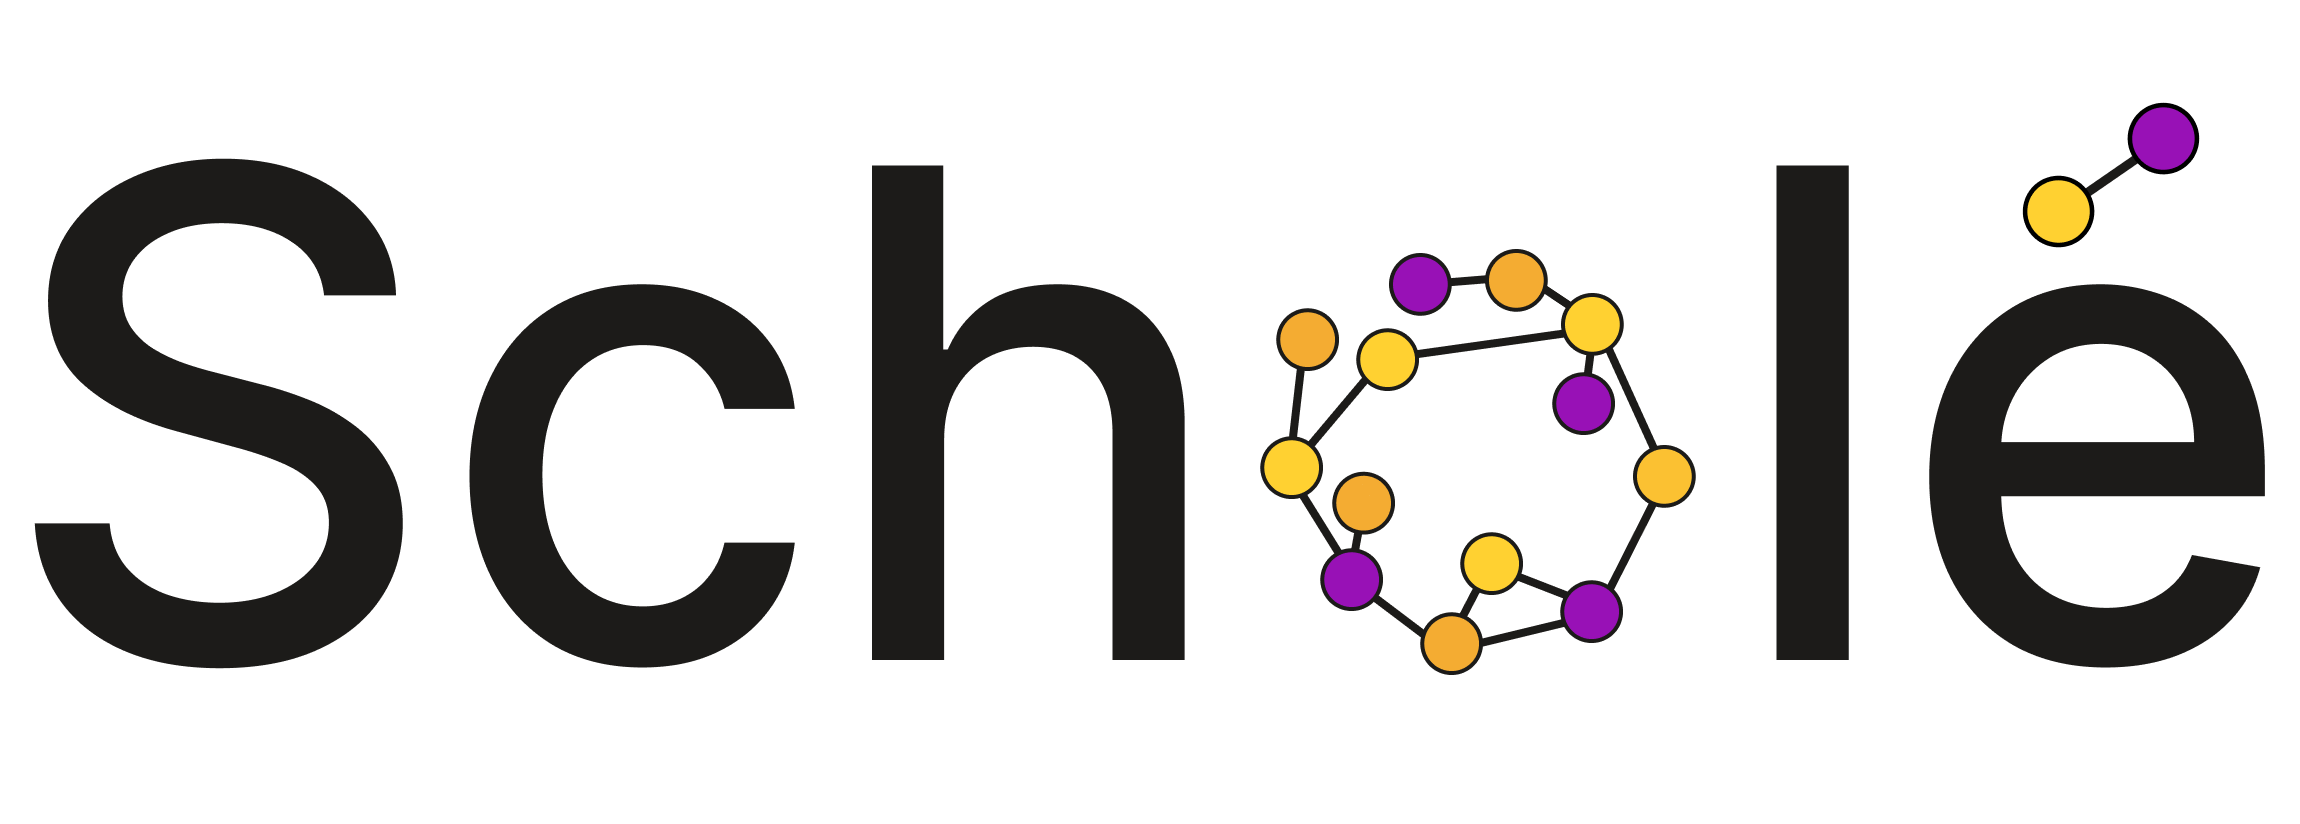
\includegraphics[width=5cm]{Images/schole.png}
    %\caption{Scholé AI | Personalized Learning at Scale}
    %\label{fig:my_label}
%\end{wrapfigure}

%Developped in collaboration with EPFL's ML4ED research lab and recognized by the 2024 Learning Engineering Tools Competition, MIT Solve, and the EPFL Ignition Grant, Schol\'e  AI is a startup committed to transforming the future of online education.

Traditional online learning platforms like Coursera and edX often suffer from high dropout rates in MOOCs, with figures reaching up to 90\% \cite{warwick65543}. Scholé tackles this challenge by providing adult learners with personalized and flexible learning paths, using multimodal content to adaptively tailor instruction to each individual's needs.

At the heart of Scholé lies Olé, an AI teaching assistant that designs personalized data science learning plans based on a team’s specific context. While large language models (LLMs) offer powerful generative capabilities, aligning their outputs with individual learner preferences remains a key challenge in educational AI, particularly when privacy must be preserved and scalability taken into account.

In this project, we explore Reinforcement Learning from Human Feedback (RLHF) \cite{ouyang2022traininglanguagemodelsfollow} as a suitable approach to align learning plans with both explicit user preferences and implicit behavioral signals. Unlike supervised fine-tuning or rule-based methods, RLHF is better suited to our setting, where feedback can be indirect, noisy, and often comparative in nature. It allows us to leverage the available signals to optimize learning plan quality in a more flexible and data-efficient way.

To preserve privacy and enhance scalability, we adapt the \textsc{FedBiscuit} framework \cite{wu2025federatedrlhfaggregatedclient}, a state-of-the-art approach for federated RLHF, to the context of personalized learning. This setup allows preference alignment across decentralized learners without centralizing sensitive data. In our setting, this is particularly important, as user interactions may be tied to confidential company-specific knowledge, making it essential to avoid exposing raw behavioral data during training.

Due to the limited availability of real user interaction data at this stage, we generate qualitative synthetic data using LLMs to simulate both explicit and implicit feedback signals. We then train personalized curriculum generators on this data using DPO-style preference learning in a federated setting. Our work demonstrates how combining RLHF, preference modeling, and federated learning can enable scalable and privacy-aware personalization for education.

This project is guided by the following research questions:

{\small
\begin{itemize}
    \item \textbf{RQ1.} How can RLHF be leveraged to personalize AI-driven learning experiences in data science while preserving user privacy?
    \item \textbf{RQ2.} How can high-quality synthetic data be generated under strict format and semantic constraints?
    \item \textbf{RQ3.} What methods can be used to evaluate the quality of both the synthetic data and the models trained using RLHF?
\end{itemize}
}

The following sections present related work, experiments, and key findings.
